\documentclass{beamer}
\usepackage{amsmath,graphics}
\usepackage{amssymb}

\usetheme{default}
\usepackage{xcolor}

\definecolor{solarizedBase03}{HTML}{002B36}
\definecolor{solarizedBase02}{HTML}{073642}
\definecolor{solarizedBase01}{HTML}{586e75}
\definecolor{solarizedBase00}{HTML}{657b83}
\definecolor{solarizedBase0}{HTML}{839496}
\definecolor{solarizedBase1}{HTML}{93a1a1}
\definecolor{solarizedBase2}{HTML}{EEE8D5}
\definecolor{solarizedBase3}{HTML}{FDF6E3}
\definecolor{solarizedYellow}{HTML}{B58900}
\definecolor{solarizedOrange}{HTML}{CB4B16}
\definecolor{solarizedRed}{HTML}{DC322F}
\definecolor{solarizedMagenta}{HTML}{D33682}
\definecolor{solarizedViolet}{HTML}{6C71C4}
%\definecolor{solarizedBlue}{HTML}{268BD2}
\definecolor{solarizedBlue}{HTML}{134676}
\definecolor{solarizedCyan}{HTML}{2AA198}
\definecolor{solarizedGreen}{HTML}{859900}
\definecolor{myBlue}{HTML}{162DB0}%{261CA4}
\setbeamercolor*{item}{fg=myBlue}
\setbeamercolor{normal text}{fg=solarizedBase03, bg=solarizedBase3}
\setbeamercolor{alerted text}{fg=myBlue}
\setbeamercolor{example text}{fg=myBlue, bg=solarizedBase3}
\setbeamercolor*{frametitle}{fg=solarizedRed}
\setbeamercolor*{title}{fg=solarizedRed}
\setbeamercolor{block title}{fg=myBlue, bg=solarizedBase3}
\setbeameroption{hide notes}
\setbeamertemplate{note page}[plain]
\beamertemplatenavigationsymbolsempty
\usefonttheme{professionalfonts}
\usefonttheme{serif}

\usepackage{fourier}

\def\vec#1{\mathchoice{\mbox{\boldmath$\displaystyle#1$}}
{\mbox{\boldmath$\textstyle#1$}}
{\mbox{\boldmath$\scriptstyle#1$}}
{\mbox{\boldmath$\scriptscriptstyle#1$}}}
\definecolor{OwnGrey}{rgb}{0.560,0.000,0.000} % #999999
\definecolor{OwnBlue}{rgb}{0.121,0.398,0.711} % #1f64b0
\definecolor{red4}{rgb}{0.5,0,0}
\definecolor{blue4}{rgb}{0,0,0.5}
\definecolor{Blue}{rgb}{0,0,0.66}
\definecolor{LightBlue}{rgb}{0.9,0.9,1}
\definecolor{Green}{rgb}{0,0.5,0}
\definecolor{LightGreen}{rgb}{0.9,1,0.9}
\definecolor{Red}{rgb}{0.9,0,0}
\definecolor{LightRed}{rgb}{1,0.9,0.9}
\definecolor{White}{gray}{1}
\definecolor{Black}{gray}{0}
\definecolor{LightGray}{gray}{0.8}
\definecolor{Orange}{rgb}{0.1,0.2,1}
\setbeamerfont{sidebar right}{size=\scriptsize}
\setbeamercolor{sidebar right}{fg=Black}

\renewcommand{\emph}[1]{{\textcolor{solarizedRed}{\itshape #1}}}

\newcommand\tay{T}
\newcommand\dd{\mathrm d}
\newcommand\eul{\mathrm e}
\newcommand\ii{\vec i}

\newcommand\cA{\mathcal A}
\newcommand\cB{\mathcal B}
\newcommand\cC{\mathcal C}
\newcommand\cD{\mathcal D}
\newcommand\cE{\mathcal E}
\newcommand\cF{\mathcal F}
\newcommand\cG{\mathcal G}
\newcommand\cH{\mathcal H}
\newcommand\cI{\mathcal I}
\newcommand\cJ{\mathcal J}
\newcommand\cK{\mathcal K}
\newcommand\cL{\mathcal L}
\newcommand\cM{\mathcal M}
\newcommand\cN{\mathcal N}
\newcommand\cO{\mathcal O}
\newcommand\cP{\mathcal P}
\newcommand\cQ{\mathcal Q}
\newcommand\cR{\mathcal R}
\newcommand\cS{\mathcal S}
\newcommand\cT{\mathcal T}
\newcommand\cU{\mathcal U}
\newcommand\cV{\mathcal V}
\newcommand\cW{\mathcal W}
\newcommand\cX{\mathcal X}
\newcommand\cY{\mathcal Y}
\newcommand\cZ{\mathcal Z}

\newcommand\fA{\mathfrak A}
\newcommand\fB{\mathfrak B}
\newcommand\fC{\mathfrak C}
\newcommand\fD{\mathfrak D}
\newcommand\fE{\mathfrak E}
\newcommand\fF{\mathfrak F}
\newcommand\fG{\mathfrak G}
\newcommand\fH{\mathfrak H}
\newcommand\fI{\mathfrak I}
\newcommand\fJ{\mathfrak J}
\newcommand\fK{\mathfrak K}
\newcommand\fL{\mathfrak L}
\newcommand\fM{\mathfrak M}
\newcommand\fN{\mathfrak N}
\newcommand\fO{\mathfrak O}
\newcommand\fP{\mathfrak P}
\newcommand\fQ{\mathfrak Q}
\newcommand\fR{\mathfrak R}
\newcommand\fS{\mathfrak S}
\newcommand\fT{\mathfrak T}
\newcommand\fU{\mathfrak U}
\newcommand\fV{\mathfrak V}
\newcommand\fW{\mathfrak W}
\newcommand\fX{\mathfrak X}
\newcommand\fY{\mathfrak Y}
\newcommand\fZ{\mathfrak Z}

\newcommand\fa{\mathfrak a}
\newcommand\fb{\mathfrak b}
\newcommand\fc{\mathfrak c}
\newcommand\fd{\mathfrak d}
\newcommand\fe{\mathfrak e}
\newcommand\ff{\mathfrak f}
\newcommand\fg{\mathfrak g}
\newcommand\fh{\mathfrak h}
%\newcommand\fi{\mathfrak i}
\newcommand\fj{\mathfrak j}
\newcommand\fk{\mathfrak k}
\newcommand\fl{\mathfrak l}
\newcommand\fm{\mathfrak m}
\newcommand\fn{\mathfrak n}
\newcommand\fo{\mathfrak o}
\newcommand\fp{\mathfrak p}
\newcommand\fq{\mathfrak q}
\newcommand\fr{\mathfrak r}
\newcommand\fs{\mathfrak s}
\newcommand\ft{\mathfrak t}
\newcommand\fu{\mathfrak u}
\newcommand\fv{\mathfrak v}
\newcommand\fw{\mathfrak w}
\newcommand\fx{\mathfrak x}
\newcommand\fy{\mathfrak y}
\newcommand\fz{\mathfrak z}

\newcommand\vA{\vec A}
\newcommand\vB{\vec B}
\newcommand\vC{\vec C}
\newcommand\vD{\vec D}
\newcommand\vE{\vec E}
\newcommand\vF{\vec F}
\newcommand\vG{\vec G}
\newcommand\vH{\vec H}
\newcommand\vI{\vec I}
\newcommand\vJ{\vec J}
\newcommand\vK{\vec K}
\newcommand\vL{\vec L}
\newcommand\vM{\vec M}
\newcommand\vN{\vec N}
\newcommand\vO{\vec O}
\newcommand\vP{\vec P}
\newcommand\vQ{\vec Q}
\newcommand\vR{\vec R}
\newcommand\vS{\vec S}
\newcommand\vT{\vec T}
\newcommand\vU{\vec U}
\newcommand\vV{\vec V}
\newcommand\vW{\vec W}
\newcommand\vX{\vec X}
\newcommand\vY{\vec Y}
\newcommand\vZ{\vec Z}

\newcommand\va{\vec a}
\newcommand\vb{\vec b}
\newcommand\vc{\vec c}
\newcommand\vd{\vec d}
\newcommand\ve{\vec e}
\newcommand\vf{\vec f}
\newcommand\vg{\vec g}
\newcommand\vh{\vec h}
\newcommand\vi{\vec i}
\newcommand\vj{\vec j}
\newcommand\vk{\vec k}
\newcommand\vl{\vec l}
\newcommand\vm{\vec m}
\newcommand\vn{\vec n}
\newcommand\vo{\vec o}
\newcommand\vp{\vec p}
\newcommand\vq{\vec q}
\newcommand\vr{\vec r}
\newcommand\vs{\vec s}
\newcommand\vt{\vec t}
\newcommand\vu{\vec u}
\newcommand\vv{\vec v}
\newcommand\vw{\vec w}
\newcommand\vx{\vec x}
\newcommand\vy{\vec y}
\newcommand\vz{\vec z}

\renewcommand\AA{\mathbb A}
\newcommand\NN{\mathbb N}
\newcommand\ZZ{\mathbb Z}
\newcommand\PP{\mathbb P}
\newcommand\QQ{\mathbb Q}
\newcommand\RR{\mathbb R}
\newcommand\RRpos{\mathbb R_{\geq0}}
\renewcommand\SS{\mathbb S}
\newcommand\CC{\mathbb C}

\newcommand{\ord}{\mathrm{ord}}
\newcommand{\id}{\mathrm{id}}
\newcommand{\pr}{\mathrm{P}}
\newcommand{\Vol}{\mathrm{vol}}
\newcommand\norm[1]{\left\|{#1}\right\|} 
\newcommand\sign{\mathrm{sign}}
\newcommand{\eps}{\varepsilon}
\newcommand{\abs}[1]{\left|#1\right|}
\newcommand\bc[1]{\left({#1}\right)} 
\newcommand\cbc[1]{\left\{{#1}\right\}} 
\newcommand\bcfr[2]{\bc{\frac{#1}{#2}}} 
\newcommand{\bck}[1]{\left\langle{#1}\right\rangle} 
\newcommand\brk[1]{\left\lbrack{#1}\right\rbrack} 
\newcommand\scal[2]{\bck{{#1},{#2}}} 
\newcommand{\vecone}{\mathbb{1}}
\newcommand{\tensor}{\otimes}
\newcommand{\diag}{\mathrm{diag}}
\newcommand{\ggt}{\mathrm{ggT}}
\newcommand{\kgv}{\mathrm{kgV}}
\newcommand{\trans}{\top}

\newcommand{\Karonski}{Karo\'nski}
\newcommand{\Erdos}{Erd\H{o}s}
\newcommand{\Renyi}{R\'enyi}
\newcommand{\Lovasz}{Lov\'asz}
\newcommand{\Juhasz}{Juh\'asz}
\newcommand{\Bollobas}{Bollob\'as}
\newcommand{\Furedi}{F\"uredi}
\newcommand{\Komlos}{Koml\'os}
\newcommand{\Luczak}{\L uczak}
\newcommand{\Kucera}{Ku\v{c}era}
\newcommand{\Szemeredi}{Szemer\'edi}

\renewcommand{\ae}{\"a}
\renewcommand{\oe}{\"o}
\newcommand{\ue}{\"u}
\newcommand{\Ae}{\"A}
\newcommand{\Oe}{\"O}
\newcommand{\Ue}{\"U}

\newcommand{\im}{\mathrm{im}}
\newcommand{\rrk}{\mathrm{zrg}}
\newcommand{\crk}{\mathrm{srg}}
\newcommand{\rk}{\mathrm{rg}}
\newcommand{\GL}{\mathrm{GL}}
\newcommand{\SL}{\mathrm{SL}}
\newcommand{\SO}{\mathrm{SO}}
\newcommand{\nul}{\mathrm{nul}}
\newcommand{\eig}{\mathrm{eig}}

\newcommand{\mytitle}{Komplexe Zahlen}

\title[Annuma]{\mytitle}
\author[Amin Coja-Oghlan]{Amin Coja-Oghlan}
\institute[Frankfurt]{JWGUFFM}
\date{}

\begin{document}

\frame[plain]{\titlepage}

\begin{frame}\frametitle{\mytitle}
	\begin{block}{Worum geht es?}
		\begin{itemize}
			\item Die komplexen Zahlen $\CC$ sind eine Erweiterung der reellen Zahlen $\RR$.
			\item Beim \Ue bergang zu den komplexen Zahlen geht allerdins die Anordnung verloren.
			\item Daf\ue r sind die komplexen Zahlen $\CC$ \emph{algebraisch abgeschlossen}.
			\item Durch die komplexen Zahlen k\oe nnen die trigonometrischen Funktionen auf die Exponentialfunktion zur\ue ckgef\ue hrt werden.
		\end{itemize}
	\end{block}
\end{frame}

\begin{frame}\frametitle{\mytitle}
	\begin{block}{Definition}
			Die Menge $\CC$ der komplexen Zahlen ist definiert als die Paare $\binom xy$ reeller Zahlen.
	\end{block}
\end{frame}

\begin{frame}\frametitle{\mytitle}
	\begin{block}{Addition und Subtraktion}
			\begin{itemize}
				\item Seien $a=\binom uv$ und $b=\binom xy$ zwei komplexe Zahlen.
			\item Wir definiern
				\begin{align*}
					a+b&=\binom{u+x}{v+y}&
					a-b&=\binom{u-x}{v-y}&
					-a&=\binom{-u}{-v}
				\end{align*}
			\end{itemize}
	\end{block}
\end{frame}

\begin{frame}\frametitle{\mytitle}
	\begin{block}{Beispiel}
			\begin{itemize}
				\item $\binom{1}2+\binom34=\binom46$
				\item $\binom12-\binom34=\binom{-2}{-2}$
				\item $\binom{-\sqrt 2}{3/4}+\binom00=\binom{-\sqrt2}{3/4}$
				\item $-\binom{-\sqrt 2}{3/4}=\binom{\sqrt2}{-3/4}$
			\end{itemize}
	\end{block}
\end{frame}

\begin{frame}\frametitle{\mytitle}
	\begin{block}{Multiplikation}
		\begin{itemize}
				\item Seien $a=\binom uv$ und $b=\binom xy$ zwei komplexe Zahlen.
				\item Wir definieren
					\begin{align*}
						a\cdot b&=\binom{u\cdot x-v\cdot y}{u\cdot y+v\cdot x}
					\end{align*}
		\end{itemize}	
	\end{block}
\end{frame}

\begin{frame}\frametitle{\mytitle}
	\begin{block}{Beispiel}
		\begin{itemize}
			\item $\binom11\cdot\binom11=\binom{1\cdot1-1\cdot1}{1\cdot1+1\cdot1}=\binom02$	
			\item $\binom10\cdot\binom{-1}{-2}=\binom{1\cdot(-1)-0\cdot(-2)}{1\cdot(-2)+0\cdot(-1)}=\binom{-1}{-2}$
			\item $\binom10\cdot\binom{x}{y}=\binom xy$
		\end{itemize}	
	\end{block}
\end{frame}

\begin{frame}\frametitle{\mytitle}
	\begin{block}{Inverse}
		\begin{itemize}
			\item F\ue r eine komplexe Zahl $a=\binom uv\neq\binom00$ definieren wir
				\begin{align*}
					a^{-1}&=\binom{u/\bc{u^2+v^2}}{-v/\bc{u^2+v^2}}
				\end{align*}
			\item Dann gilt
				\begin{align*}
					a\cdot a^{-1}&=\binom10
				\end{align*}
		\end{itemize}	
	\end{block}
\end{frame}

\begin{frame}\frametitle{\mytitle}
	\begin{block}{Beispiel}
		\begin{itemize}
			\item $\binom11^{-1}=\binom{1/\bc{1^2+1^2}}{-1/\bc{1^2+1^2}}=\binom{1/2}{-1/2}$ und
				\begin{align*}
					\binom11\cdot\binom{1/2}{-1/2}=\binom{1\cdot\frac{1}{2}-1\cdot\bcfr{-1}2}{1\cdot\frac{1}{2}+1\cdot\frac{-1}{2}}=\binom10
				\end{align*}
			\item $\binom 70^{-1}=\binom{7/(7^2+0^2)}{-0/(7^2+0^2)}=\binom{1/7}0$
			\item $\binom 07^{-1}=\binom{0/(7^2+0^2)}{-7/(7^2+0^2)}=\binom0{-1/7}$
		\end{itemize}	
	\end{block}
\end{frame}

\begin{frame}\frametitle{\mytitle}
	\begin{block}{Konjugation}
		\begin{itemize}
			\item Sei $\binom xy\in\CC$.
			\item Das \emph{Konjugierte} von $\binom xy$ ist definiert als
				\begin{align*}
					\overline{\binom xy}=\binom x{-y}
				\end{align*}
		\end{itemize}	
	\end{block}
\end{frame}

\begin{frame}\frametitle{\mytitle}
	\begin{block}{Beispiel}
		\begin{itemize}
			\item $\overline{\binom12}=\binom1{-2}$
			\item $\overline{\binom70}=\binom70$
			\item $\overline{\binom0{-\pi}}=\binom0{\pi}$
		\end{itemize}	
	\end{block}
\end{frame}

\begin{frame}\frametitle{\mytitle}
	\begin{block}{Der komplexe Betrag}
		\begin{itemize}
			\item Sei $\binom xy\in\CC$.
			\item Wir definieren
				\begin{align*}
					\abs{\binom xy}=\sqrt{x^2+y^2}\in\RRpos
				\end{align*}
		\end{itemize}	
	\end{block}
\end{frame}

\begin{frame}\frametitle{\mytitle}
	\begin{block}{Beispiel}
		\begin{itemize}
			\item $\abs{\binom11}=\sqrt{1^2+1^2}=\sqrt2$
			\item $\abs{\binom70}=\sqrt{7^2+0^2}=7$
			\item $\abs{\binom0{-7}}=\sqrt{0^2+(-7)^2}=7$
		\end{itemize}	
	\end{block}
\end{frame}
\begin{frame}\frametitle{\mytitle}
	\begin{block}{Rechenregeln f\ue r die komplexen Zahlen}
		F\ue r alle $a,b,c\in\CC$ gelten die folgenden Rechenregeln:
		\begin{description}
			\item[Kommutativgesetze:] 
					\begin{align*}
						a+b&=b+a,&a\cdot b&=b\cdot a
			\end{align*}
			\item[Assoziativgesetze:]	
				\begin{align*}
					(a+b)+c&=a+(b+c),&(a\cdot b)\cdot c&=a\cdot(b\cdot c)
				\end{align*}
			\item[Neutrales Element:]
				\begin{align*}
					\binom 00+a&=a,&\binom10\cdot a&=a
				\end{align*}
			\item[Distributivgesetz:]
				\begin{align*}
					a\cdot(b+c)&=a\cdot b+a\cdot c
				\end{align*}
		\end{description}
	\end{block}
\end{frame}

\begin{frame}\frametitle{\mytitle}
	\begin{block}{Rechenregeln f\ue r die komplexen Zahlen (fortgesetzt)}
		\begin{description}
			\item[Negatives Element:] 
					\begin{align*}
						a+(-a)=0
			\end{align*}
			\item[Inverses Element:]	
				falls $a\neq\binom00$, gilt
				\begin{align*}
					a\cdot a^{-1}=\binom10
				\end{align*}
			\item[Konjugation:] 
				\begin{align*}
					\overline{\overline a}&=a\\ a\cdot\overline a&=\binom{|a|^2}0
				\end{align*}
		\end{description}
	\end{block}
\end{frame}

\begin{frame}\frametitle{\mytitle}
	\begin{block}{Rechenregeln f\ue r die komplexen Zahlen (fortgesetzt)}
		\begin{description}
			\item[Betrag:] 
				\begin{align*}
					|a|&=0\qquad\Leftrightarrow\qquad a=\binom00\\
					|a\cdot b|&=|a|\cdot|b|\\
					|a+b|&\leq|a|+|b|
				\end{align*}
		\end{description}
	\end{block}
\end{frame}

\begin{frame}\frametitle{\mytitle}
	\begin{block}{Einbettung der reellen Zahlen}
		\begin{itemize}
			\item wie \alert{identifizieren} die reelle Zahl $x$ mit der komplexen Zahl
				\begin{align*}
				\binom x0
				\end{align*}
			\item dann k\oe nnen wir $\RR$ als Teilmenge von $\CC$ auffassen
			\item insbesondere werden aus den reellen Zahlen $0$ und $1$ die komplexen Zahlen
				\begin{align*}
					0&=\binom00&1&=\binom10
				\end{align*}
			\item f\ue r diese gelten die \ue blichen Rechenregeln
				\begin{align*}
					0+a&=a&&1\cdot a=a&&(a\in\CC)
				\end{align*}
		\end{itemize}
	\end{block}
\end{frame}

\begin{frame}\frametitle{\mytitle}
	\begin{block}{Die imagin\ae re Einheit}
		\begin{itemize}
			\item Wir haben gesehen, da\ss\ $1=\binom10\in\CC$ das neutrale Element bzgl.\ der Multiplikation ist.
			\item Auch die komplexe Zahl
				\begin{align*}
				\ii=\binom01
				\end{align*}
				spielt eine ausgezeichnete Rolle; sie wird die \emph{imagin\ae re Einheit} genannt.
			\item Es gilt
				\begin{align*}
					\ii^2&=\binom01\cdot\binom01=\binom{0\cdot0-1\cdot1}{0\cdot1+1\cdot0}=\binom{-1}0=-1
				\end{align*}
		\end{itemize}
	\end{block}
\end{frame}

\begin{frame}\frametitle{\mytitle}
	\begin{block}{Die imagin\ae re Einheit (fortgesetzt)}
		\begin{itemize}
			\item In $\CC$ hat also $-1$ die Quadratwurzel $\ii$.
			\item Eine zweite Quadratwurzel von $-1$ ist die Zahl
				\begin{align*}
					-\ii=\binom0{-1}
				\end{align*}
			\item Die quadratische Gleichung $X^2+1=0$ hat also zwei komplexe Nullstellen $\pm\ii$.
		\end{itemize}
	\end{block}
\end{frame}

\begin{frame}\frametitle{\mytitle}
	\hfill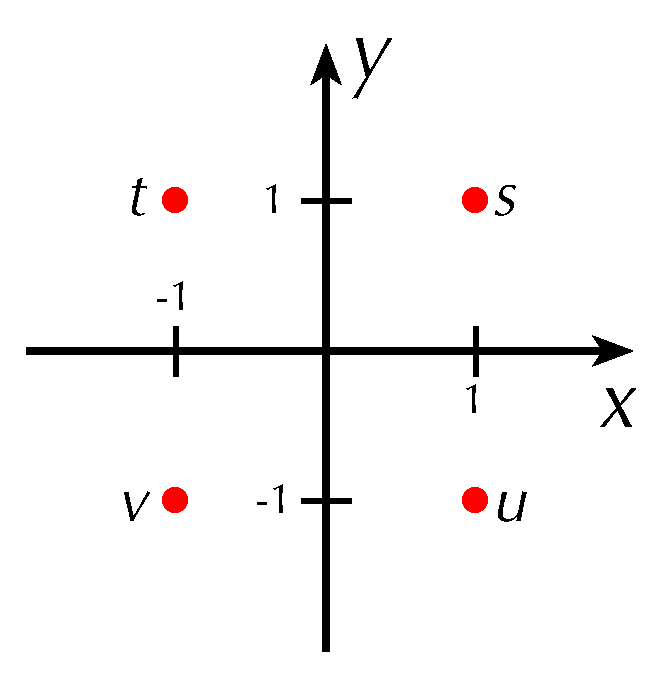
\includegraphics[height=30mm]{pics/vectors.pdf}
	\begin{block}{Die Gau\ss sche Zahlenebene}
		\begin{itemize}
			\item mit den Konventionen $1=\binom 10$ und $\ii=\binom 01$ k\oe nnen wir jede komplexe Zahl schreiben als
				\begin{align*}
				\binom xy=x\cdot 1+y\cdot\ii=x+y\ii
				\end{align*}
			\item wir nennen daher die $y$-Achse auch die \emph{imagin\ae re Achse} und die $x$-Achse die \emph{reelle Achse}.
		\end{itemize}
	\end{block}
\end{frame}

\begin{frame}\frametitle{\mytitle}
	\hfill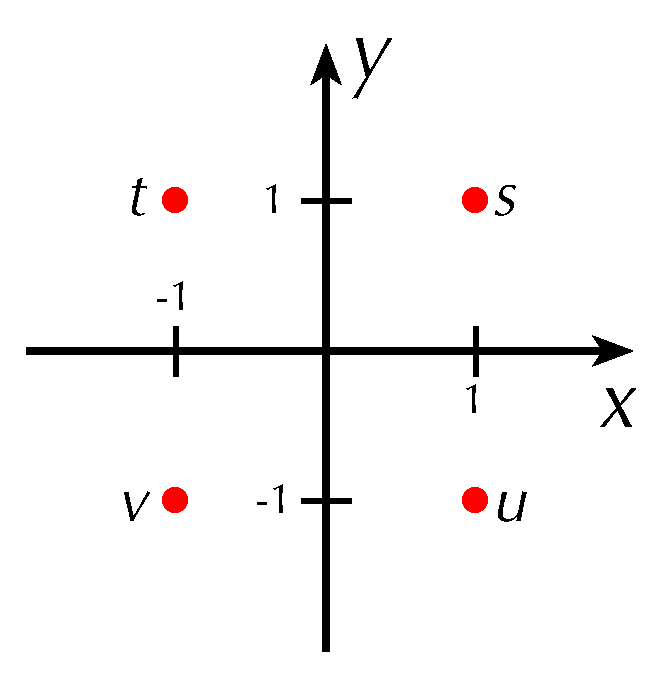
\includegraphics[height=30mm]{pics/vectors.pdf}
	\begin{block}{Die Gau\ss sche Zahlenebene (fortgesetzt)}
		\begin{itemize}
			\item der \emph{Realteil} einer komplexen Zahl ist definiert als
				\begin{align*}
					\Re(x+y\ii)=x.
				\end{align*}
			\item der \emph{Imagin\ae rteil} einer komplexen Zahl ist definiert als
				\begin{align*}
					\Im(x+y\ii)=y.
				\end{align*}
		\end{itemize}
	\end{block}
\end{frame}

\begin{frame}\frametitle{\mytitle}
	\hfill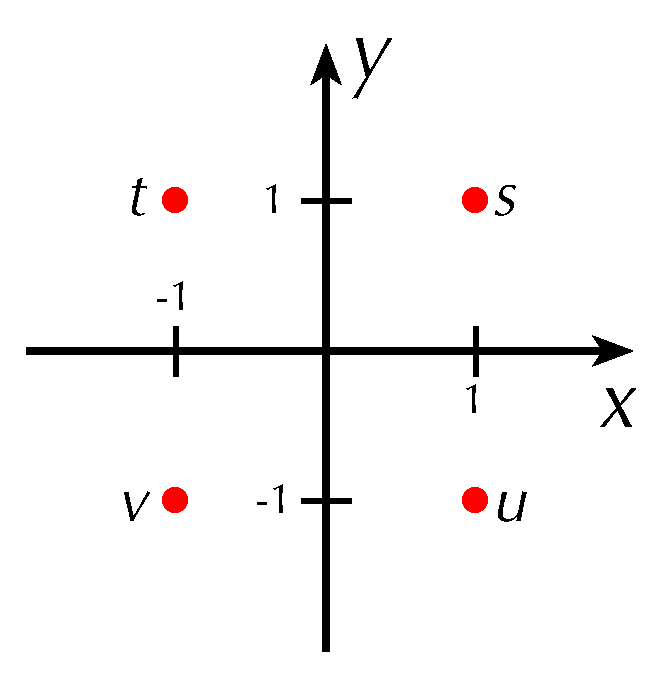
\includegraphics[height=30mm]{pics/vectors.pdf}
	\begin{block}{Die Gau\ss sche Zahlenebene (fortgesetzt)}
		\begin{itemize}
			\item wenn Rechenaufgaben mit komplexen Zahlen gestellt werden, ist das Ergebnis immer in der Form
				\begin{align*}
					\Re(a)+\ii\Im(a)
				\end{align*}
				anzugeben.
		\end{itemize}
	\end{block}
\end{frame}

\begin{frame}\frametitle{\mytitle}
	\begin{block}{Beispiel}
		\begin{itemize}
			\item wir berechnen $\frac{1-\ii}{2+\ii}$:
				\begin{align*}
					\frac{1-\ii}{2+\ii}&=(1-\ii)\cdot(2+\ii)^{-1}=(1-\ii)\cdot\frac{2-\ii}{2^2+1^2}\\
									   &=\frac{(1-\ii)(2-\ii)}{5}=\frac{2-\ii-2\ii+\ii^2}{5}\\
									   &=\frac{2-3\ii-1}{5}=\frac{1-3\ii}{5}=\frac{1}{5}-\frac{3}{5}\ii.
				\end{align*}
			\item Also
				\begin{align*}
					\Re\bcfr{1-\ii}{2+\ii}&=\frac{1}{5}&\Im\bcfr{1-\ii}{2+\ii}&=-\frac{3}{5}.
				\end{align*}
		\end{itemize}
	\end{block}
\end{frame}

\begin{frame}\frametitle{\mytitle}
	\begin{block}{Fundamentalsatz der Algebra}
		\begin{itemize}
			\item Sei $$f(z)=\sum_{i=0}^ka_kz^k$$ 
				ein Polynom mit $k\geq1$, $a_0,\ldots,a_k\in\CC$, $a_k\neq0$.
			\item Dann gibt es eine komplexe Zahl $b$, so da\ss
				\begin{align*}
					f(b)=0.
				\end{align*}
			\item \itshape Jedes nichttriviale Polynom hat eine komplexe Nullstelle.
		\end{itemize}
	\end{block}
\end{frame}

\begin{frame}\frametitle{\mytitle}
	\begin{block}{Fundamentalsatz der Algebra (fortgesetzt)}
		\begin{itemize}
			\item Daraus folgt, da\ss\ jedes komplexe Polynom in Linearfaktoren zerf\ae llt, d.h.\ es gibt $b_1,\ldots,b_k,c\in\CC$, so da\ss
				\begin{align*}
					f(x)=c\prod_{i=1}^k(x-b_i)
				\end{align*}
		\end{itemize}
	\end{block}
\end{frame}

\begin{frame}\frametitle{\mytitle}
	\begin{block}{Beispiel}
		\begin{itemize}
			\item Das Polynom $$f(x)=x^2+1$$ hat keine reelle Nullstelle, aber die zwei komplexen Nullstellen $\pm\ii$.
			\item Wir erhalten die Faktorisierung
				\begin{align*}
					f(x)=(x+\ii)(x-\ii).
				\end{align*}
		\end{itemize}
	\end{block}
\end{frame}

\begin{frame}\frametitle{\mytitle}
	\begin{block}{Komplexe Grenzwerte}
		\begin{itemize}
			\item Sei $(a_n)_n$ eine Folge komplexer Zahlen.
			\item Wir sagen, die Folge \emph{konvergiert} gegen $z\in\CC$, falls
				\begin{align*}
					\lim_{n\to\infty}|a_n-z|=0.
				\end{align*}
			\item Wir k\oe nnen daher auch von Reihen im Komplexen reden.
		\end{itemize}
	\end{block}
\end{frame}

\begin{frame}\frametitle{\mytitle}
	\begin{block}{Komplexe Grenzwerte (fortgesetzt)}
		\begin{itemize}
			\item Sei $(a_n)_n$ eine Folge komplexer Zahlen.
			\item Die Folge konvergiert genau dann gegen $z\in\CC$, wenn
				\begin{align*}
					\lim_{n\to\infty}\Re(a_n)=\Re(z)\mbox{ und }\lim_{n\to\infty}\Re(a_n)=\Im(z).
				\end{align*}
			\item Die Folge konvergiert also genau dann, wenn die beiden Folgen $(\Re(a_n))_n$ und $(\Im(a_n))_n$ konvergieren.
		\end{itemize}
	\end{block}
\end{frame}

\begin{frame}\frametitle{\mytitle}
	\begin{block}{Die Exponentialreihe}
		\begin{itemize}
			\item Die Reihe
				\begin{align*}
					\sum_{k=0}^\infty\frac{z^k}{k!}
				\end{align*}
				konvergiert f\ue r alle $z\in\CC$.
			\item Wir definieren daher die \emph{Exponentialfunktion}
				\begin{align*}
				 \exp(z)=	\sum_{k=0}^\infty\frac{z^k}{k!}
				\end{align*}
		\end{itemize}
	\end{block}
\end{frame}

\begin{frame}\frametitle{\mytitle}
	\begin{block}{Die trigonometrischen Funktionen}
		\begin{itemize}
			\item Die komplexen Reihen
				\begin{align*}
					\cos(z)&=\sum_{k=0}^\infty\frac{(-1)^kz^{2k}}{(2k)!}\\
					\sin(z)&=\sum_{k=0}^\infty\frac{(-1)^kz^{2k+1}}{(2k+1)!}
				\end{align*}
				konvergieren ebenfalls f\ue r alle $z\in\CC$.
			\item Unter Verwendung der Formel $\ii^2=-1$ ergibt sich daher
				\begin{align*}
					\exp(\ii x)&=\cos(x)+\ii\sin(x)&&(x\in\RR).
				\end{align*}
		\end{itemize}
	\end{block}
\end{frame}

\begin{frame}\frametitle{\mytitle}
	\begin{block}{Rechenregeln f\ue r die Exponentialfunktion}
		\begin{itemize}
			\item Es gilt
				\begin{align*}
					\exp(a+b)&=\exp(a)\cdot\exp(b)&&(a,b\in\CC)
				\end{align*}
			\item F\ue r alle $z\in\CC$ gilt
				\begin{align*}
					|\exp(z)|=\exp(\Re(z))
				\end{align*}
		\end{itemize}
	\end{block}
\end{frame}

\begin{frame}\frametitle{\mytitle}
	\begin{block}{Polarkoordinaten}
		\begin{itemize}
			\item Zu jeder komplexen Zahl $z$ gibt es eine Zahl $t\in(-\pi,\pi]$ mit
				\begin{align*}
					z=|z|\exp(\ii t).
				\end{align*}
			\item Diese Zahl $t$ nennt man das \emph{Argument} $\mbox{arg}(z)$.
		\end{itemize}
	\end{block}
\end{frame}

\begin{frame}\frametitle{\mytitle}
	\begin{block}{Zusammenfassung}
		\begin{itemize}
			\item Komplexe Zahlen sind eine Erweiterung der reellen Zahlen
			\item Fundamentalsatz der Algebra
			\item Wir haben Folgen und Reihen im komplexen definiert und insbesondere die Exponentialreihe kenengelernt.
			\item Es ist nicht m\oe glich, die komplexen Zahlen anzuordnen.
		\end{itemize}
	\end{block}
\end{frame}

\end{document}
